\subsection{Gauss Map}

In one dimension, the curvature is the rate of change of the tangent vector.
For an orientable surface $S$, we consider the rate of change of the normal vector.
This vector is given by the map  $N:S\to \Sp^2$ that sends each
normal in $S$ to the corresponding point on $\Sp^2$ is
the \EMPH{Gauss map}.
The determinant of the derivative of the Gauss map, $dN(p)$ quantifies the rate of change of
the normal vector ($dN$ is often called the \emph{Weingarten map} \cite{Crane:2013}).
Thus, $dN_p:T_p(S)\to T_{N(p)}(\Sp^2)$, but since $T_p(S)$ and $T_{N(p)}(\Sp^2)$
are parallel we can define $dN_p$ to be a linear map on $T_p(S)$.
The determinant of $dN(p)$ is equal to \EMPH{Gaussian curvature}.



\begin{example}[Stereographic Projection \cite{christian-notes}]\label{ex:stereo}
Consider the two sphere with the north pole removed $\Sp^2 \setminus (0,0,1)$,
stereographic projection is a bijection between the points on $\Sp^2 \setminus (0,0,1)$ to the $\R^2$.
Consider a line from the north pole $(0,0,1)$ that intersects $(x,y,z)\in \Sp^2$ parametrized by 
$p(t)=(1-t)(0,0,1)+t(x,y,z)$. By considering the $z$ coordinate we determine the $t$ value where this line
intersects $\R^2$, namely $t=\frac{1}{1-z}.$
This gives the desired map shown in \figref{stereo} and in equation form
$$p(x,y,z)\to \left(\frac{x}{1-z},\frac{y}{1-z}\right).$$

\begin{figure}[htb]
	\centering
	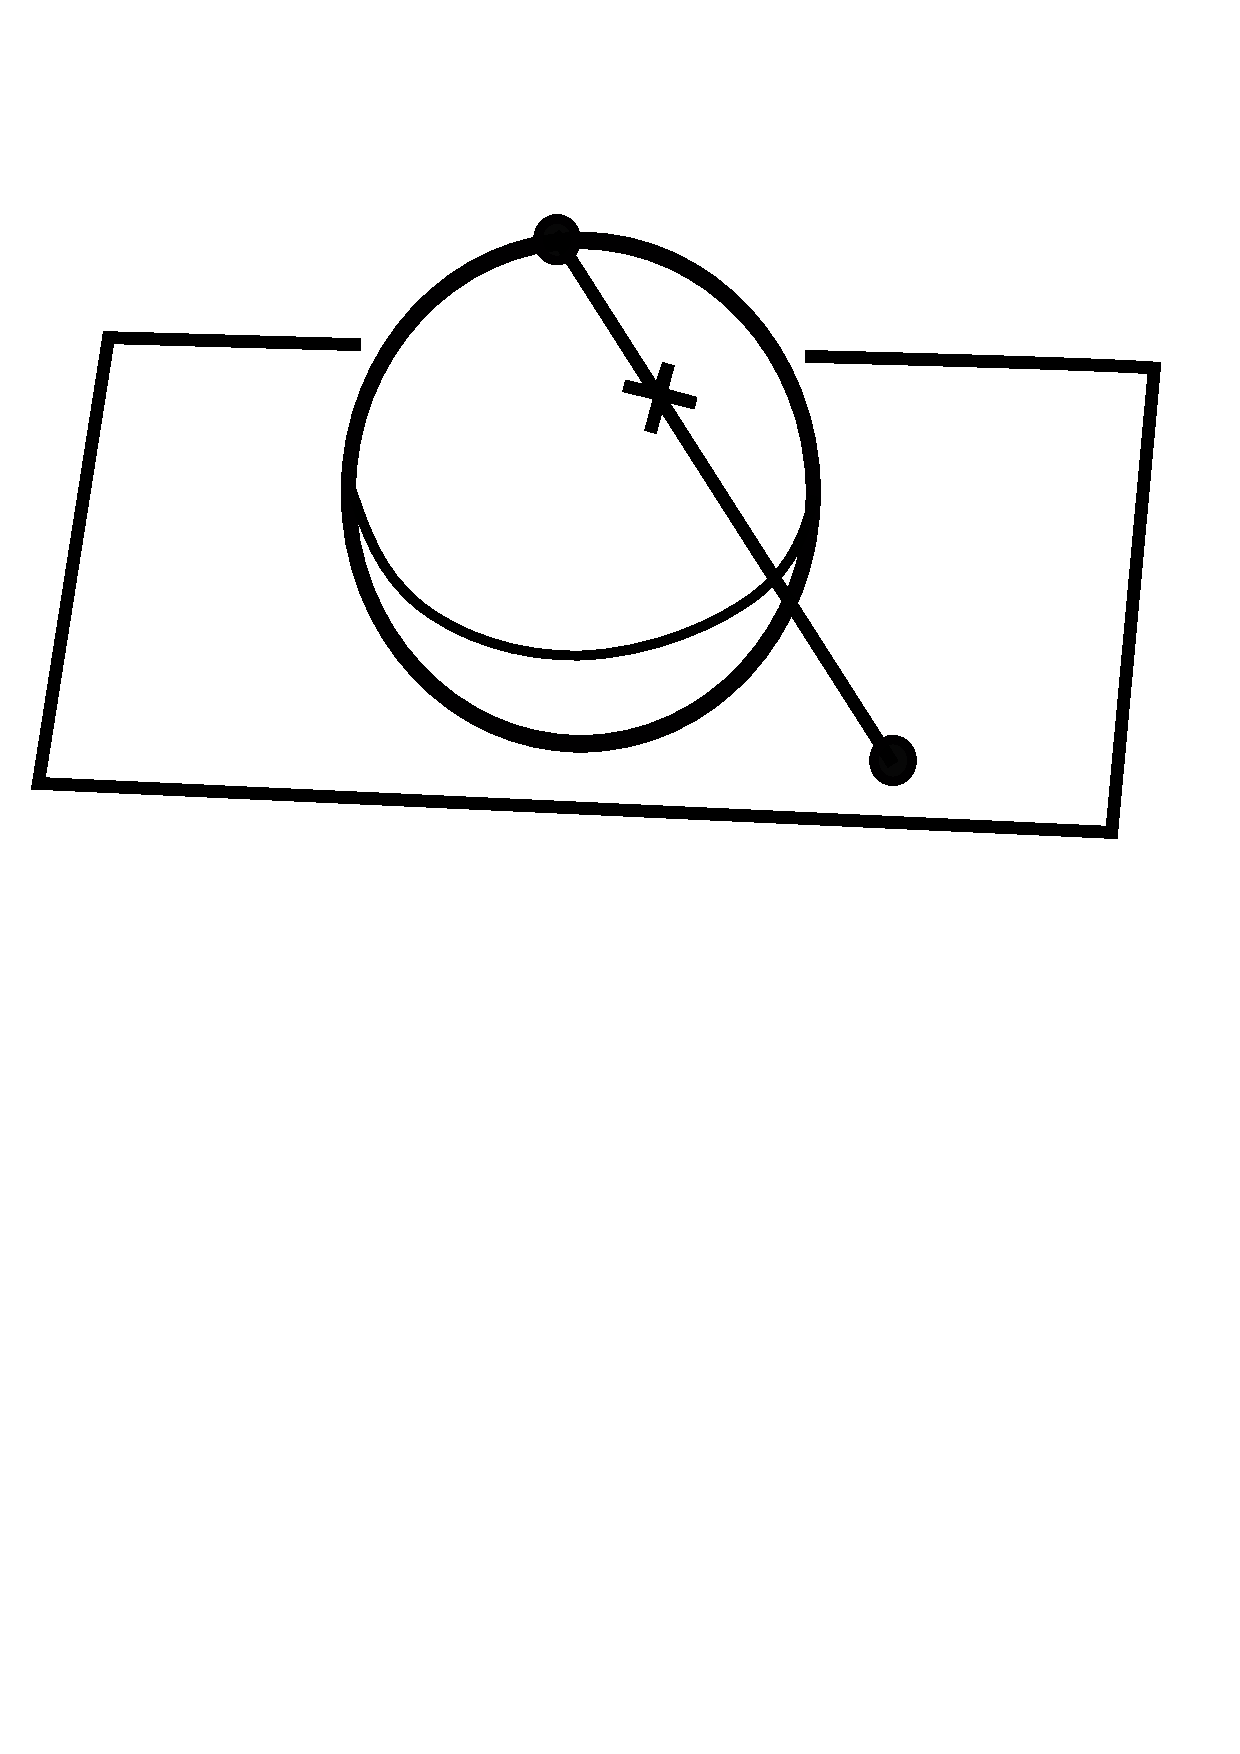
\includegraphics[width=.3\textwidth]{curvature/stereo}
	\caption{A point on the sphere is mapped to a point on the plane by stereographic projection.}
	\label{fig:stereo}
\end{figure}
	
The inverse is given by $p^{-1}:\R^2\to \R^3$

	\begin{equation}\label{eqn:stereo}
		p^{-1}(u,v)=\left(\frac{2u}{u^2+v^2+1},\frac{2v}{u^2+v^2+1},\frac{u^2+v^2-1}{u^2+v^2+1}\right).	
	\end{equation}
To compute the first fundamental form of $p^{-1}(u,v)$ we take the partial derivatives

$$p^{-1}_u=\left(\frac{2v^2-2u^2+2}{(u^2+v^2+1)^2},\frac{-4uv}{(u^2+v^2+1)^2},\frac{4v}{(u^2+v^2+1)^2}\right)$$
and 
$$p^{-1}_v=\left(\frac{-4uv}{(u^2+v^2+1)^2},\frac{2v^2-2u^2+2}{(u^2+v^2+1)^2},\frac{4v}{(u^2+v^2+1)^2}\right).$$
Then, after some algebra,
$$E=p^{-1}_u\cdot p^{-1}_u=\frac{4}{(u^2+v^2+1)^2}$$
$$F=p^{-1}_v\cdot p^{-1}_v=\frac{4}{(u^2+v^2+1)^2}$$
and
$$M=p^{-1}_u\cdot p^{-1}_v=0.$$

We can use the first fundamental form to compute
the  arc length of circles on the sphere parallel to the $xy$ plane with fixed height $z=c$ for $-1<c<1$.
This length can be computed using
the pythagorean theorem. We will see that using stereographic projection
and the first fundamental form we get the same answer.


The arc length of a parameterized curve $u=u(t), v=v(t)$ on a regular surface,
can be computed using the first fundamental form.  Let
$s$ denote the arc length, then 
$$ds=\bigg | \frac{dr}{dt}\bigg | dt = \bigg | r_u\frac{du}{dt}+r_v\frac{dv}{dt}\bigg |dt
=\sqrt{(r_u^2 du^2+2r_ur_v du dv + r_v^2dv^2)}.$$
Next, use the map $p$ to map such a circle to the plane.
Using \eqnref{stereo}, our circle on the sphere maps 
to a circle in the plane because
	$$p^{-1}(u,v)=\frac{u^2+v^2-1}{u^2+v^2+1}=c$$
and we can compute the radius in terms of $c$
\begin{equation}\label{eqn:radius}
	u^2+v^2=\frac{1+c}{1-c}=k^2.
\end{equation}
	
In the plane, $u^2+v^2=k^2$ can be parameterized
as $$\gamma(t)=(k\cos(t),k\sin(t))$$ with $0\leq t\leq 2\pi.$
So our curve becomes $p^{-1}\circ \gamma(t)$ on the sphere.
Computing the partial derivatives of $\gamma(t)$ gives
$$\gamma_u'=-k\sin(t)\hspace{1.3cm}  \gamma_v'=k\cos(t).$$
Now we use the first fundamental form

$$\int_{p^{-1}}\gamma ds=\int_{0}^{2\pi} ||(p^{-1}\circ \gamma)'(t)dt=\int_0^{2\pi}\sqrt{E(\gamma_u'(t))^2+2M\gamma_u'\gamma_v'+
F(\gamma_v'(t))^2}dt.$$
Substituting and simplifying using $E=F$ we obtain
$$\int_0^{2\pi}\frac{2k}{k^2+1}dt=\frac{4\pi k}{k^2+1}.$$
Simplifying further using \eqnref{radius}  our arc length is
$$2\pi\sqrt{1-c^2}.$$

\end{example}

\todo{Do we need this? Let $S_1$ and $S_2$ be two surfaces with $\sigma:V\subset S_1\to S_2$ a differentiable map.
At $p\in S_1$ the map $d\sigma_p:T_p(S_1)\to T_{\sigma(p)}(S_2)$ is called the
\EMPH{differential} of $\sigma$ at $p$.}


Given two curves on the sphere that intersect linearly independently at a point $p$, 
stereographic projection preserves the angle between the curves.
Maps that preserve angles in this way are called \EMPH{conformal}.